\section{Theoretical basis of AI}
\subsection{AI algorithms for classification}
From a theoretical point of view many AI algorithms are formulated in terms of classification, i.e. a pattern recognition problem can be formulated as a classification problem. 
\\\\
A data set consists from cases (objects) and each case is characterised by some features, each case can be represented by a vector of features such that $\overrightarrow{x} = (x_1,x_2,...,x_p)$  each vector can be considered as a dot in p-dimensional space and all cases together form a cloud. If we Assume that each vector belongs to some class, the number of classes is M. The goal is to find a classifier that assigns to each case a label of some class.
\subsubsection{What a computer can see}
An image classifier takes a single image and assigns probabilities to labels. For an image of size $248\times400$ pixels and three colour channels, the image will consist of 297,600 numbers where each number is an an integer in a range from 0 to 255, our task if turn these numbers into a label.
\subsection{Data pre-processing}
There are four common forms of data pre-processing: centering, normalisation, dimensionality reduction, noise cancelling. To understand these procedure we assume that our data has a random nature and we use probability theory and statistics to deal with random variable and data analysis. 
\\\\
A Data matrix $X$, where we will assume that $X$ is of size $[n,p]$ (where $n$ is the number of data ( cases), $p$ is the dimensionality of the feature vector).

\subsection{Normal distribution}
A continuous random variable $X$ which is bell-shaped and has mean (expectation) $\mu$ and standard deviation $\sigma$ is said to follow a Normal Distribution with
parameters $\mu$ and $\sigma$.
\\\\
In shorthand, $X \sim \mathcal{N}(\mu,\,\sigma^{2})\,.$
This may be given in \emph{standardised} form by using the transformation
\begin{equation}
    z = \frac{z - \mu}{\sigma} \rightarrow x = \sigma z+ \mu \text{, where } Z \sim \mathcal{N}(0,\,1)\,.
\end{equation}
The normal distribution is important because of the Central Limit Theorem which states that a sum of arbitrary random variables will have a distribution that is approximately normal. 
\subsection{Bivariate normal distribution }
The multivariate normal distribution is a generalisation of the univariate normal to two or more variables, Each element of a normally distributed random vector has a univariate normal distribution. In the simplest case there is no correlation among variables, and elements of the vectors are independent univariate normal random variables. 

\begin{figure}[htbp]
    \def\centerx{2}
    \def\centery{-1}
    
    \centering
    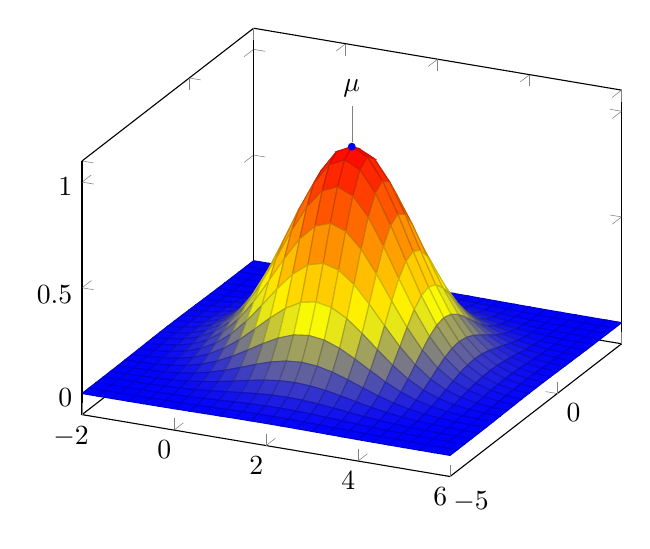
\begin{tikzpicture}
        \begin{axis}
        \addplot3[surf,domain=-2:6,domain y=-5:3] 
            {exp(-( (x-\centerx)^2 + (y-\centery)^2)/3 )};
        \node[circle,inner sep=1pt,fill=blue,pin=90:$\mu$] 
            at (axis cs:\centerx,\centery,1) {};
        \end{axis}
    \end{tikzpicture}
    \caption{Bivariate normal distribution 3D perceptive}
    \label{fig:my_label}
\end{figure}
\begin{figure}[htbp]
    \def\centerx{2}
    \def\centery{-1}
    \centering
    \begin{tikzpicture}
        \begin{axis}[view={0}{90},axis equal]
        \addplot3[contour gnuplot,domain=-2:6,domain y=-5:3] 
            {exp(-( (x-\centerx)^2 + (y-\centery)^2)/3 )};
        \node[circle,inner sep=1pt,fill=blue,pin=90:$\mu$] 
            at (axis cs:\centerx,\centery,1) {};
        \end{axis}
    \end{tikzpicture}
    \caption{Bivariate normal distribution 2D perceptive}
    \label{fig:my_label}
\end{figure}
$p$ is the correlation $-1 \leq p \leq 1$ 
\begin{itemize}
    \item $p = 0$ means that the varables are independent
    \item $p = +1$ means that the variables are linearly dependent
    \item $p = -1$ means also the linear dependence but the increase of one variable is associated with the decrease of an other.
\end{itemize}
\subsection{Statistics: Random sample}
Statistics is an interface between the probability theory and data, it provides multiple procedures for data analysis. In statistics the data set is a sample, this sample should be chosen in a proper way and correctly represent a random variable which we would like to estimate.
\subsection{Parameter estimators}
Data analysis is based of statistical estimator of the random variable $X$, i.e. for sample $X = (x_1,x_2,...,x_n)$, 
\\\\
The estimator of the mean is
\begin{equation}
  \Bar{X} = \frac{1}{n}\sum_{i=1}^{n} x_i.
\end{equation}
The estimator of the variance is 
\begin{equation}
  S_x^2 = \frac{1}{n} {\sum_{i=1}^{n} (x_i - \Bar{X})^2}.
\end{equation}
The estimator of the standard deviation is 
\begin{equation}
    S_x = \sqrt{\frac{1}{n} {\sum_{i=1}^{n} (x_i - \Bar{X})^2}}
\end{equation}
Now consider the bivariate random variable $(X,Y) = \{(x_i,y_i)\},i = 1,2,...,n$
\\\\
The estimator of the covariance is 
\begin{equation}
    cov(X,Y) = \frac{1}{n-1} {\sum_{i=1}^{n} (x_i - \Bar{X})}(y_i - \Bar{Y})}
\end{equation}
The estimator of the correlation is 
\begin{equation}
    p = \frac{cov(X,Y)}{S_x S_y}
\end{equation}
\subsection{Data Centering}
Mean subtraction is the most common form of pre-processing, it involves subtracting $\mu$ across every individual feature in the data and has the geometric interpretation of centering the cloud of data around the origin along every dimension. 
\subsection{Data normalisation}
Normalisation referees to normalising the data dimensions so that they are approximately the same scale. There are two common ways of achieving this normalisation
\begin{enumerate}
    \item To divide each dimension by its standard deviation, once it has been zero centered
    \item normalised each dimension so that the min and max along the dimension is -1 and 1 respectively
\end{enumerate}
It only makes sense to apply this pre-processing if you have a reason to believe that different input features have different scales, but thy should be approximately equal importance to the learning algorithm. In the cases of images the relative scales of pixels are already approximately equal, so it is not strictly necessary to perform this addition pre-processing step.